\documentclass[12pt]{article}

\usepackage{amsmath}
\usepackage[authoryear,round]{natbib}
\usepackage{hyperref}



\textwidth=6.2in
\textheight=8.5in
\oddsidemargin=.1in
\evensidemargin=.1in
\headheight=-.3in

\newcommand{\scscst}{\scriptscriptstyle}
\newcommand{\scst}{\scriptstyle}
\newcommand{\Rfunction}[1]{{\texttt{#1()}}}
\newcommand{\Rmethod}[1]{{\texttt{#1}}}  
\newcommand{\Rclass}[1]{{\texttt{#1}}}
\newcommand{\Robject}[1]{{\texttt{#1}}}
\newcommand{\Rpackage}[1]{{\textit{#1}}}
\newcommand{\code}[1]{{\texttt{#1}}}
\bibliographystyle{plainnat}

\title{Outline: Analysis of High Throughput Flow Cytometry Data using \Rpackage{plateCore}}

%%%%%%%%%%%%%%%%%%%%%%%%%%%%%%%%%%%%%%%%%%%%%%%%%%%%%%%%%%%%%%%%%%%%%%%%%%%
\usepackage{/usr/local/lib/R/share/texmf/Sweave}
\begin{document}
\maketitle

\tableofcontents

%%%%%%%%%%%%%%%%%%%%%%%%%%%%%%%%%%%%%%%%%%%%%%%%%%%%%%%%%%%%%%%%%%%%%%%%%%%%%%%%%%%%%%%%%%%%%%%%%%%%%%%%%%%%%%%%%%%%%%%%%%%%%%%%%%%
\section{Abstract}
\Rpackage{plateCore} is a Bioconductor packaged created to make processing and analysis of large, complex flow cytometry (FCM) datasets
in R easier. High throughput flow studies are often run in a 96 or 384-well plate format, with a number of different samples, 
controls, and antibodies-dye conjugates present on the plate. Analyzing the output from the cytometer requires keeping track of the contents
of each well, matching sample wells with control wells, gating each well/channel separately, making the appropriate plots, assessing quality, and
summarizing the results. \Rpackage{plateCore} extends the \Rpackage{flowCore} and \Rpackage{flowViz} packages to work on
\Rclass{flowPlate} objects that represent these large flow datasets. For those familiar with\\
\Rpackage{flowCore} and \Rpackage{flowViz}, the gating (filtering), transformation, and other data manipulations for \Rclass{flowPlates} 
are very similar to \Rclass{flowSets}. 

In this document we show how use \Rpackage{plateCore} to analyze a publicly available blood dataset for expression of cell surface markers. 
This peripheral blood mononucleocyte (PBMC) data was generated using BD FACS\texttrademark CAP screening to look at the expression profiles of 189 
different human markers (add reference). The raw PBMC data is read into R using \Rpackage{flowCore}, and then the filtering and 
threshold gating are performed in \Rpackage{plateCore}. The output is the fraction of positive (expressing) cells for
each marker, which is then compared to results from expert manual analysis.

%%%%%%%%%%%%%%%%%%%%%%%%%%%%%%%%%%%%%%%%%%%%%%%%%%%%%%%%%%%%%%%%%%%%%%%%%%%%%%%%%%%%%%%%%%%%%%%%%%%%%%%%%%%%%%%%%%%%%%%%%%%%%%%%%%
\section{Introduction}
Analysis of flow cytometry high content screening (FC-HCS) experiments requires a systematic approach to
preprocessing, gating (i.e., filtering), and summarizing large amounts of data. Ideally these steps would be automated,
allowing analysis pipelines to be robust, objective, and match the high-throughput capacity of modern cytometers. 
Unfortunately, current approaches to FC-HCS analysis methods are semi-automated at best,
often requiring significant manual intervention to identify cells of interest and set the appropriate gates. 
Since the manual contribution is subjective and prone to error when working with large numbers of samples, it
is desirable to develop programmatic approaches to process the data.

Flow cytometry packages available through the Bioconductor project provide an open analysis platform that
can be used by cytometrists, bioinformaticians, and statisticians to develop new analysis approaches that
enable automated processing. The \Rpackage{flowCore} package contains the framework for importing, transforming, gating, and
organizing raw flow cytometry data. \Rpackage{flowViz} supports sophisticated visualizations based on Trellis displays. 
\Rpackage{flowClust} implements model-based clustering approaches for automated gating. The combination of
these packages provides a set of freely available, flexible, and computationally efficient FC-HCS tools.

\Rpackage{plateCore} provides a convenient way to manage the sample annotation associated with complex FC-HCS experiments, and
to access the functionality in other Bioconductor flow packages. 
The progression from raw FCM data files to a completed \Rpackage{plateCore} analysis is shown in Figure~\ref{fig:analysis}.
Since the layout of FC-HCS plates often changes from experiment
to experiment, the annotation for each well needs to be customized for each
\Rclass{flowPlate}. \Rpackage{plateCore} uses an approach that is very similar to the cell-based high throughput screening \Rpackage{cellHTS2} package (insert ref),
where users must provide a \textit{plate configuration} file for each dataset. Once the cell level data has
been analyzed in \Rpackage{plateCore}, the summary well information (i.e., percentage of positive cells and median
signal intensities) can be imported into tools like \Rpackage{cellHTS2}, since FC-HCS experiments are just one 
type of cell-based high throughput screens.


\begin{figure}
\centering
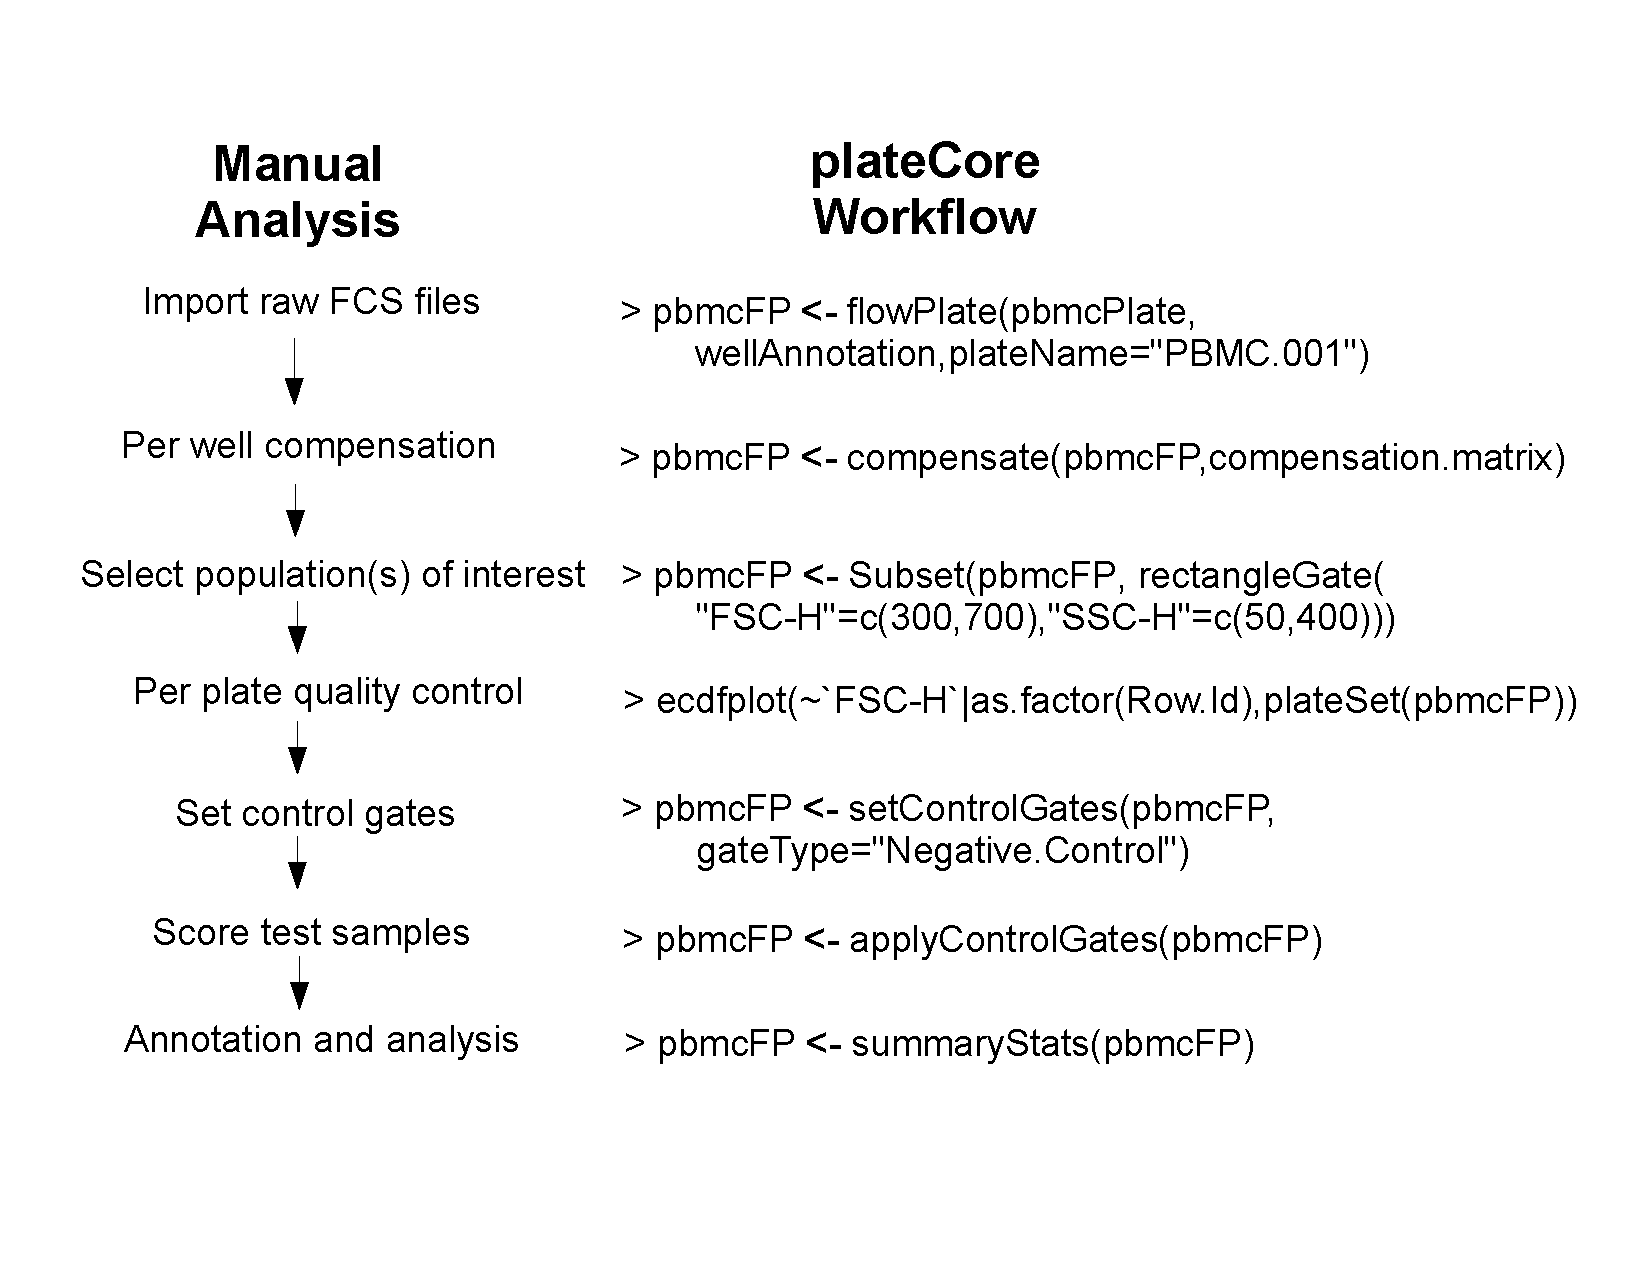
\includegraphics[width=7in,height=6in]{analysisSteps.pdf}
\caption{Typical plateCore workflow on the left, and examples of each step from a sample analysis are shown on the right.
Generating reports and plots is a multi-step that typically involves merging output from several plates, and the required
code is not shown here.
If necessary, the threshold control gates created automatically from setControlGates are adjusted based on input from flow experts. 
These new gates are established based on the gap between negative control wells and positive test samples, whereas the automated
control gates were set using only negative control wells.}
\label{fig:analysis}
\end{figure}
 
%%%%%%%%%%%%%%%%%%%%%%%%%%%%%%%%%%%%%%%%%%%%%%%%%%%%%%%%%%%%%%%%%%%%%%%%%%%%%%%%%%%%%%%%%%%%%%%%%%%%%%%%%%%%%%%%%%%%%%%%%%%%%%%%%%%
\clearpage
\section{Example Data}
The PBMC dataset used in this example is available for download from ficcs.org as the "plateData.tar.gz" file. The data consists
of 5 different peripheral blood mononucleocyte (PBMC) samples that were analyzed with 189 different antibodies on 96-well plates. Each plate has a set of
unstained, isotype, and control wells. Antibodies and isotype controls are arrayed 3 per well, and the data was compensated
on the cytometer. The \textit{plate configuration} is also included in the archive as \textit{maskPlateDesc.csv} (Note: I need
to update the description so it's compatible with the latest version of plateCore).
Unfortunately, the antibody names have been masked since the layout of the plate is proprietary. (Although
I'm cautiously optimistic that we will be able to release more information about the experiment).

%%%%%%%%%%%%%%%%%%%%%%%%%%%%%%%%%%%%%%%%%%%%%%%%%%%%%%%%%%%%%%%%%%%%%%%%%%%%%%%%%%%%%%%%%%%%%%%%%%%%%%%%%%%%%%%%%%%%%%%%%%%%%%%%%%%
\section{Analysis}
FCS files for each plate are imported in R using \Rpackage{flowCore}, and a \Robject{flowPlate} named platePBMCraw is created by integrating
the \textit{plate configuration} with the \Robject{flowSet}. The data in this experiment has already been compensated on
the cytometer, so there is no need to correct for spillover in R. This analysis will focus on lymphoctyes, which
will be selected using a forward (FSC) and side-scatter (SSC) morphology gate (Figure ~\ref{fig:morphGate}).
The \textit{Subset} function is used to select cells inside a rectangular gate, which separates the lymphocytes
from the monocytes, red blood cells, and debris.
\begin{Schunk}
\begin{Sinput}
> platePBMC <- Subset(platePBMCraw,
+ 		rectangleGate("FSC-H"=c(300,700),"SSC-H"=c(50,400)))	
\end{Sinput}
\end{Schunk}

After the lymphocytes have been filtered, the plate is then checked for fluidic events.
These fluidic events can cause a temporary shift in the cytometer detector readings, and affected wells need
to be identified and either corrected or removed from the analysis. The \Rfunction{qaProcess.timeline} from
the \Rpackage{flowQ} package can be used to search for fluidic events in \Rclass{flowSets} by looking for shifts in specific channels over time that
are above some predetermined threshold. Fluidic events can also often be identified by plotting the emprical cumulative density plots of FSC
values for each well, and looking for distributions shifted relative to other wells (Figure ~\ref{fig:fluidic}).



\begin{figure}
\centering
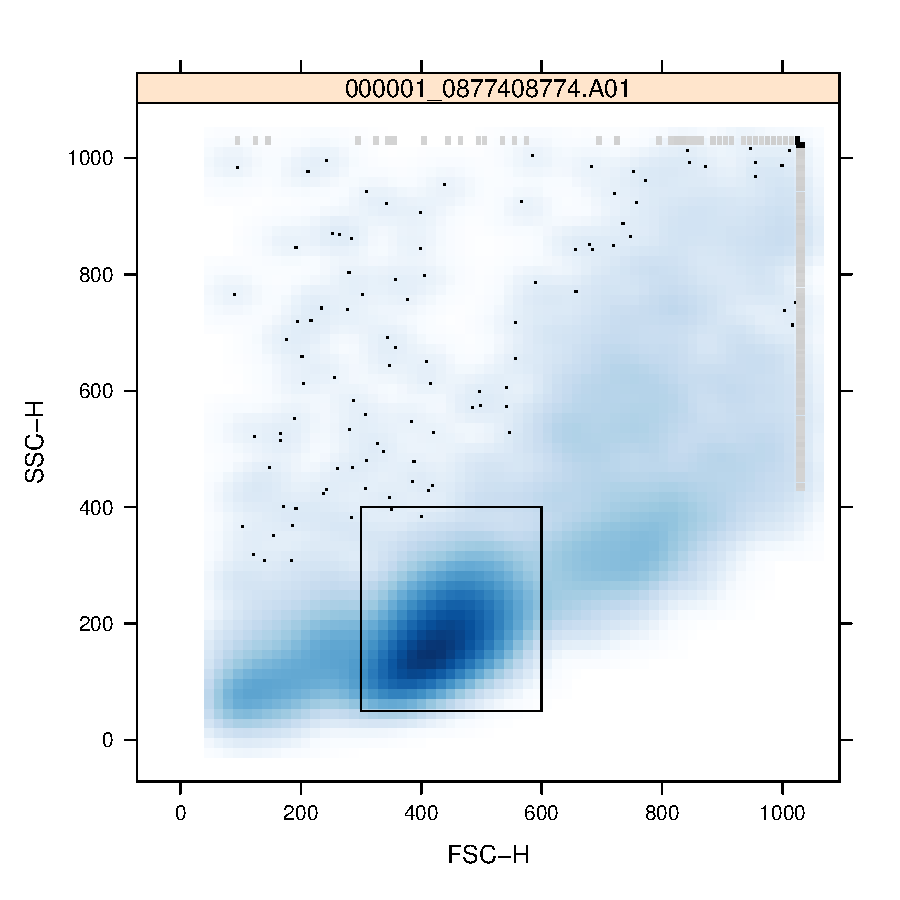
\includegraphics{outline-morphGate}
\caption{A \Rpackage{flowCore} rectangleGate used to select lymphocytes from PBMC data. The gate is displayed using the xyplot function from \Rpackage{flowViz}}
\label{fig:morphGate}
\end{figure}

\begin{figure}
\centering
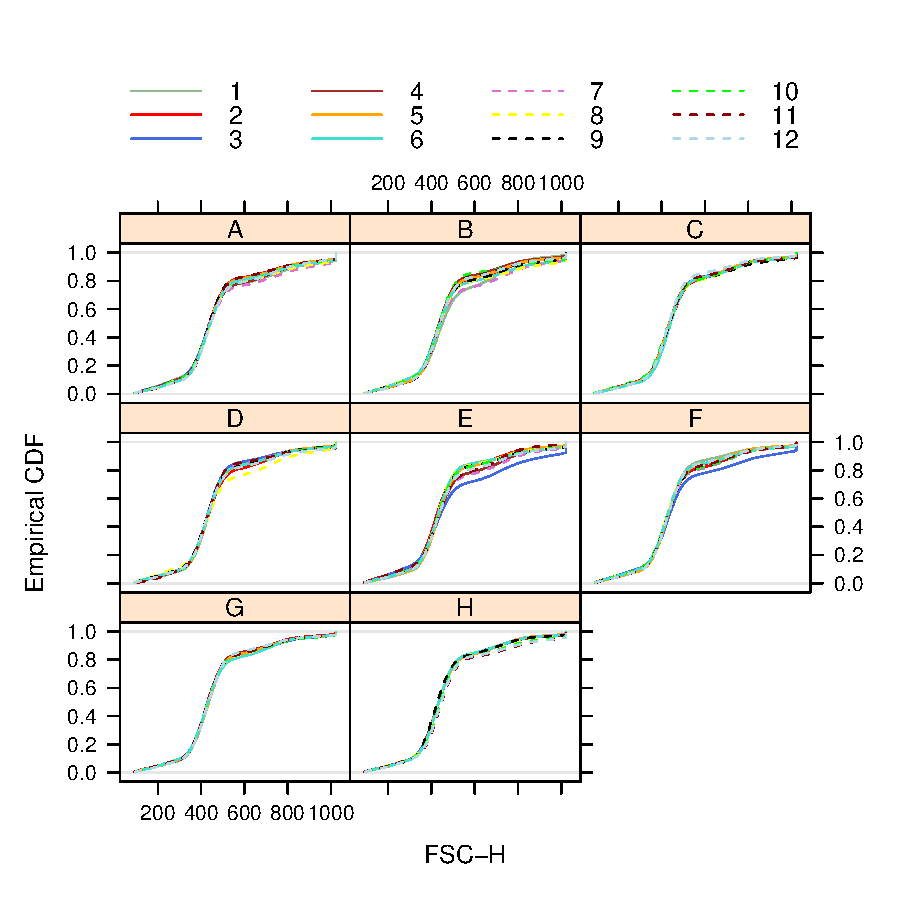
\includegraphics{outline-fluidic}
\caption{Empirical cumulative distribution function (ecdf) plots of FSC-H values for Rows A thru H. There are 12 columns in each row.
Fluidic events will often show up as a shift in the distribution of FSC-H values. 
Based on this plot wells E03 and F03 were manually checked, but the differences were not large enough to change fluorescence values.}
\label{fig:fluidic}
\end{figure}

\clearpage
Once the plate has passed quality control
checks, the next step is setting the control gate to establish the cutoff between positive and negative cells.
Ideally this expression threshold would be established using known positive and negative samples, but such information is
usually not available. Instead, the expression cutoff is generally set according to negative controls. 
For example, \Rpackage{plateCore} supports creating thresholds according to either unstained, unstimulated, isotype, 
or fluorescence minus one (FMO) controls. One-dimensional expression thresholds are initially set using
the setControlGates function. 
\begin{Schunk}
\begin{Sinput}
> platePBMC <- setControlGates(platePBMC,gateType="Negative.Control",numMads=6)
\end{Sinput}
\end{Schunk}
The "numMads" parameter sets the value of the control gate at 6 median absolute deviations (MADs) above 
the media fluorescence intensity (MFI) the control gate. The resulting gate for isotype well A03 and its
associated test wells is shown in Figure~\ref{fig:isoGate}.
\Rpackage{flowCore} and \Rpackage{flowClust} potentially offer
more robust methods of establishing this threshold using kernel density approaches, but setting the
gate at 3 to 6 MADs on linear scale signals often works well in practice for screening quality experiments.

Once the Negative.Control gates have been created and applied, we can then use the \Rfunction{summaryStats} to calculate different
metrics of interest from the \Rclass{flowPlate}. Running \Rfunction{applyControlGates} and \Rfunction{summaryStats} on \Robject{platePBMC}, 
\begin{Schunk}
\begin{Sinput}
> platePBMC <- applyControlGates(platePBMC)
> platePBMC <- summaryStats(platePBMC)
\end{Sinput}
\end{Schunk}
will result in additional columns created in the \Robject{wellAnnotation} object associated with this
particular \Robject{flowPlate}.  
These new columns include percentage of cells above the Negative.Control gate (Percent.Positive),
the number of cells in the raw data (Total.Events), the number of positive cells (Positive Count),
the median fluorescence intensity (MFI), and the ratio of the test well MFI to the MFI of the negative
control well (MFI.Ratio). In this PMBC example a number of the samples are heterogeneous, so the MFI and MFI.Ratio
may not be helpful since they are based on all the cells in a well, and not just the positive cells.


\begin{figure}
\centering
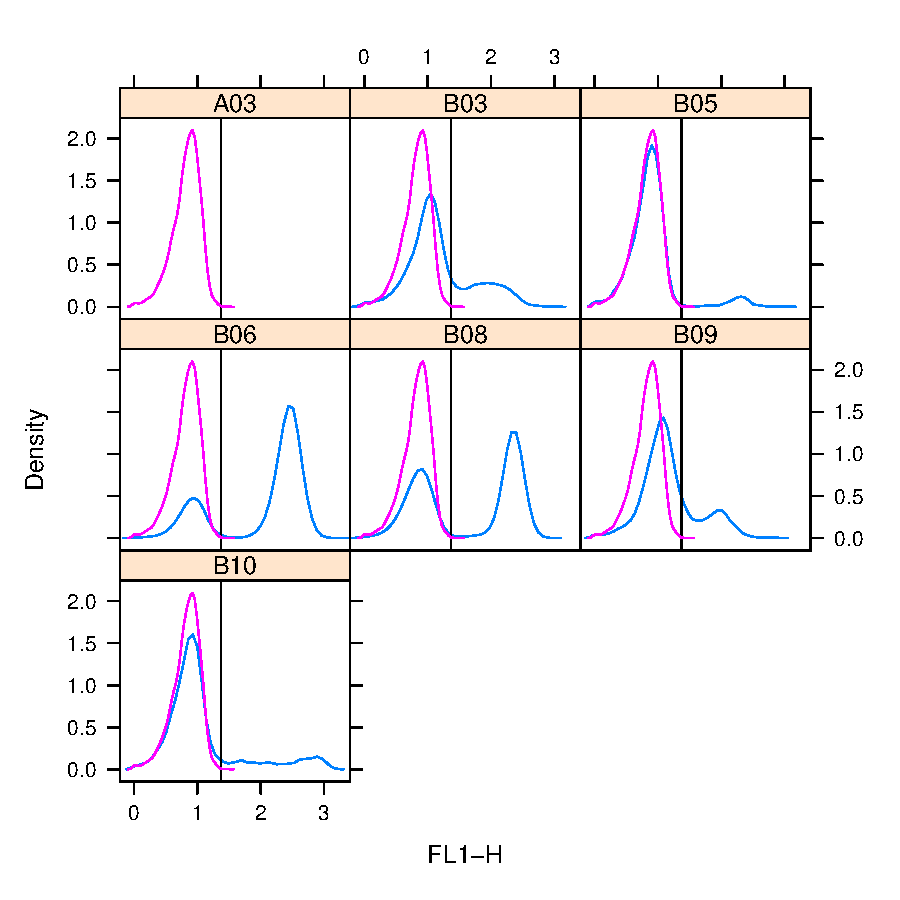
\includegraphics{outline-isoGate}
\caption{Density plots for the A03 isotype well and the associated test wells. Isotype results are shown in magenta while the test samples
are in blue. The vertical bar indicates the negative control gate, estimated using the setControlGates function with numMads=6. This
plot was created using the densityplot function specific to \Robject{flowPlates} from \Rpackage{plateCore}.}
\label{fig:isoGate}
\end{figure}

\clearpage
The wellAnnotation \Robject{data.frame} associated with each analyzed \Robject{flowPlate} can then be exported from R for
use in other programs. Sample output for well B10 in this analysis is given in Table~\ref{tab:wellAnno}. Threshold
gates created using the isotype control wells are included in the \emph{Negative.Control.Gate} column, allowing the gating to be replicated on other
software platforms.

\begin{table}[ht]
\begin{center}
\begin{tabular}{r|ccc}
  \hline
Column & B10 FL2-H &  B10 FL1-H & B10 FL4-H \\
    \hline
  Well.Id & B10 & B10 & B10 \\
  Sample.Type & Test & Test & Test \\
  Ab.Name & Cdbd28 & Cdbd29 & Cdbd30 \\
  Channel & FL2-H & FL1-H & FL4-H \\
  Negative.Control & A03 & A03 & A03 \\
  plateName & PBMC.001 & PBMC.001 & PBMC.001 \\
  name & 0877408774.B10 & 0877408774.B10 & 0877408774.B10 \\
  Negative.Control.Gate & 24 & 23 & 68 \\
  Percent.Positive &  1 & 15 &  0 \\
  Total.Count & 7598 & 7598 & 7598 \\
  Positive.Count &   58 & 1187 &    6 \\
  MFI &  4.0 &  8.2 & 11.8 \\
  MFI.Ratio & 0.64 & 1.14 & 0.78 \\
   \hline
\end{tabular}
\caption{Output for well B10 from the wellAnnotation \Robject{data.frame} associated with the PBMC \Robject{flowPlate}.}
\label{tab:wellAnno}
\end{center}
\end{table}

%%%%%%%%%%%%%%%%%%%%%%%%%%%%%%%%%%%%%%%%%%%%%%%%%%%%%%%%%%%%%%%%%%%%%%%%%%%%%%%%%%%%%%%%%%%%%%%%%%%%%%%%%%%%%%%%%%%%%%%%%%%%%%%%%%%
\clearpage
\section{Results}

FCM files from 5 PBMC plates that had been analyzed using BD FACS$^{\text{TM}}$ CAP were processed using the method
described in the analysis section. The resulting \Robject{flowPlates} were stored in \emph{RData} files so that individual plots
can be made without rerunning the analysis. The \Robject{wellAnnotation} for each \Robject[flowPlate} was then merged
into a single \Robject{data.frame}, containing the percent positive results from each plate. These values can then visualized
using microarray tools in R (Figure~\ref{fig:pbmcHeat}). 

Once a marker of interest has been identified, the next step is usually to make density or dotplots of the signals from each
plate. Although these plots can be created individually, it is more convenient to have a combined data object so that results 
from multiple \Robject{flowPlates} can be quickly summarized. \Rpackage{plateCore} supports combining \Robject{flowPlates} using
the \Rfunction{fpbind} function. 
\begin{Schunk}
\begin{Sinput}
> virtPlate <- fpbind(plate1,plate2,plate3,plate4,plate5)
\end{Sinput}
\end{Schunk}
This virtual plate can then be used to make histograms for particular markers, such as CDbd69 which showed variable levels of
expression between the different donors (Figure~\ref{fig:pbmcCDbd69}). 
\begin{Schunk}
\begin{Sinput}
> densityplot(~ `FL2-H` | as.factor(plateName),
+ 	virtPlate,filterResult="Negative.Control")
\end{Sinput}
\end{Schunk}

\begin{figure}
\centering
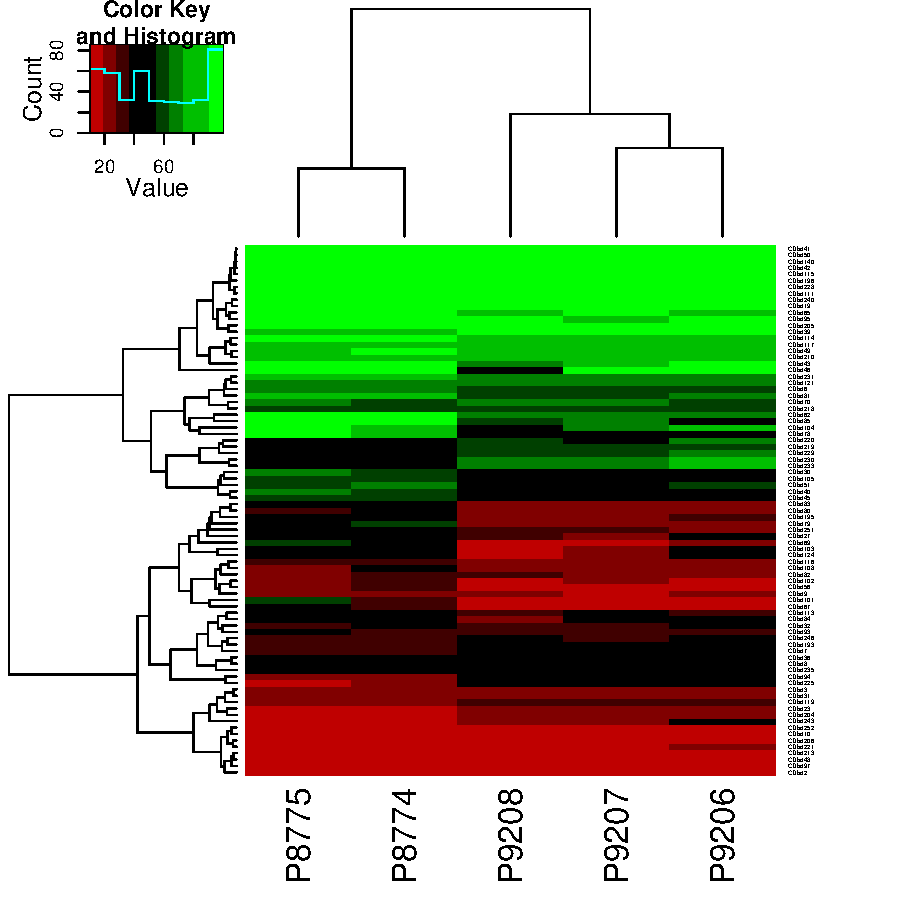
\includegraphics{outline-pbmcHeat}
\caption{Heatmap showing the percentage of positive cells from the 5 different PBMC lymphocyte plates. Only the 83 markers
that had $\ge$ 10\% positive cells are shown here.}
\label{fig:pbmcHeat}
\end{figure}

\begin{figure}
\centering
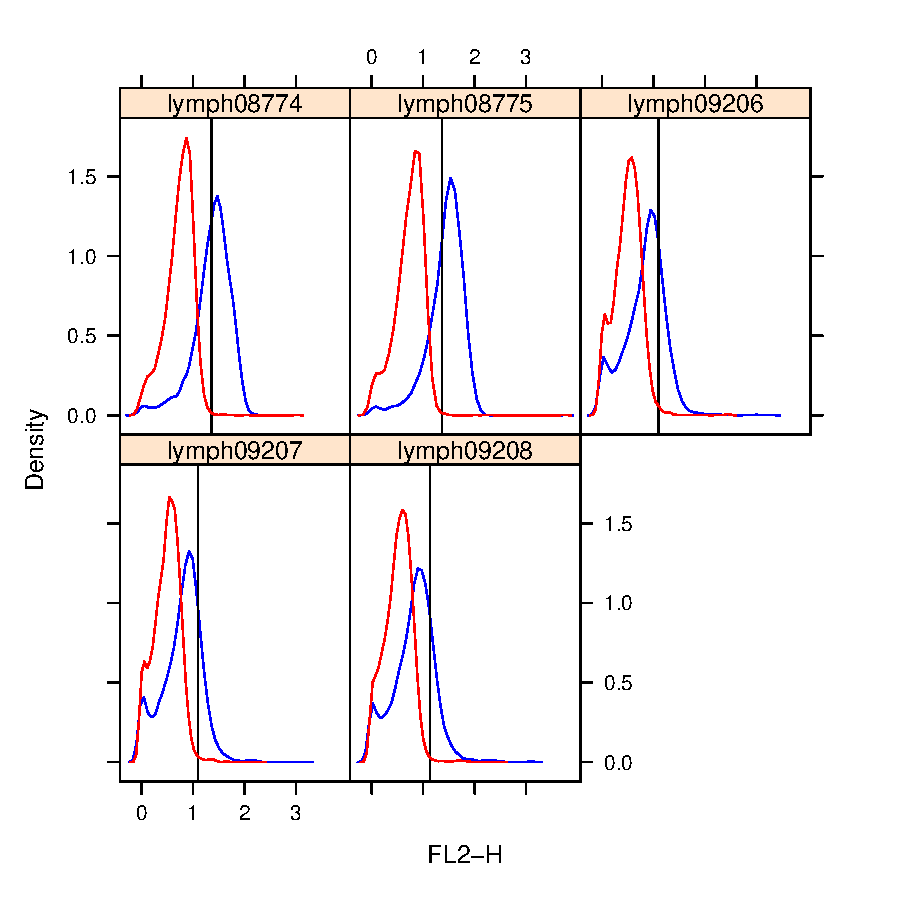
\includegraphics{outline-pbmcCDbd69}
\caption{Dotplots for CDbd69, which is differentially expressed between the 5 PBMC plates. Isotypes are shown in green and
test wells are in magenta.}
\label{fig:pbmcCDbd69}
\end{figure}

%%%%%%%%%%%%%%%%%%%%%%%%%%%%%%%%%%%%%%%%%%%%%%%%%%%%%%%%%%%%%%%%%%%%%%%%%%%%%%%%%%%%%%%%%%%%%%%%%%%%%%%%%%%%%%%%%%%%%%%%%%%%%%%%%%%
\clearpage
\section{Comparison to Manual Analysis}

The 5 pmbc plates were also analyzed using FlowJo$^{\text{TM}}$, which is one of more popular FCM data analysis programs.
BD FACS$^{\text{TM}}$ CAP is designed as a screening tool to help identify markers for additional analysis. Since it is 
not practical to have controls specific to each of the 189 antibody-dye conjugates, isotypes were chosen according to the
most common antibody subtypes. Cytometry experts initially set gates according to the isotype controls, and then move the
gates based on positive and negative test samples. Figure~\ref{} shows how the results from FlowJo$^{\text{TM}}$ compare to \Rpackage{plateCore}.

\begin{figure}
\centering
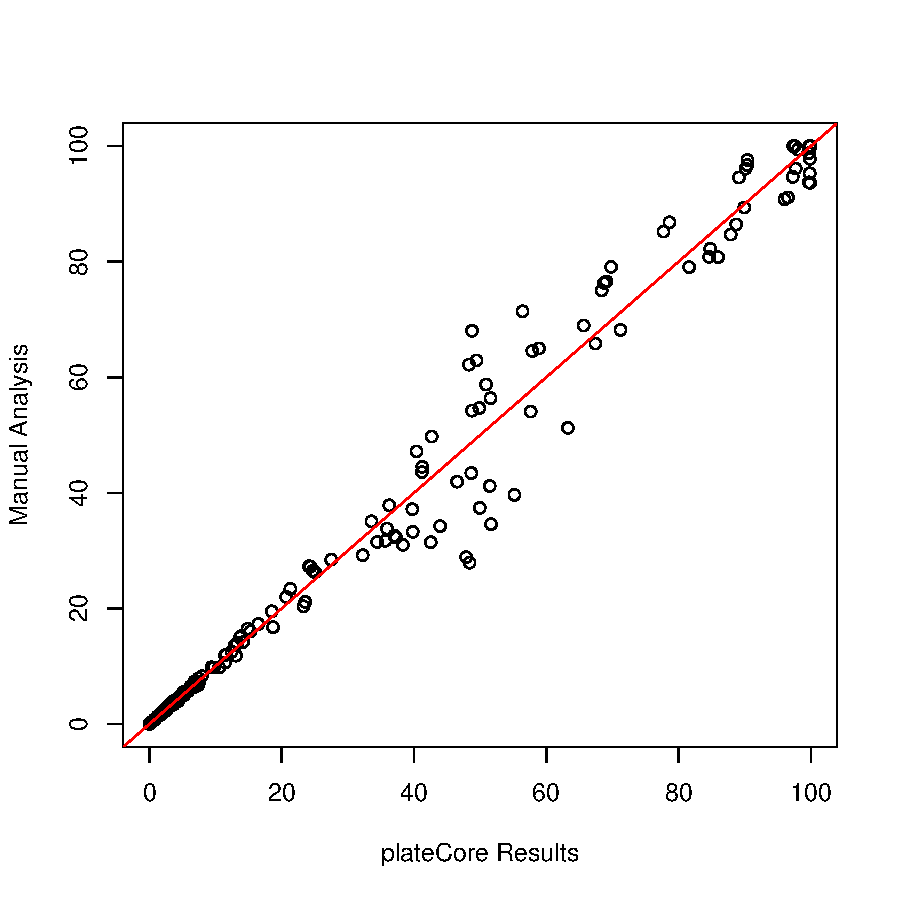
\includegraphics{outline-pcVSman}
\caption{Percent positive results for 189 markers analyzed using either \Rpackage{plateCore} or manually using FlowJo$^{\text{TM}}$.}
\label{fig:pcVSman}
\end{figure}

%%%%%%%%%%%%%%%%%%%%%%%%%%%%%%%%%%%%%%%%%%%%%%%%%%%%%%%%%%%%%%%%%%%%%%%%%%%%%%%%%%%%%%%%%%%%%%%%%%%%%%%%%%%%%%%%%%%%%%%%%%%%%%%%%%%
\clearpage
\section{Conclusions}

The PBMC example shows that a complex analysis of a 96-well plate, stained with 189 antibodies,
can be constructed in 15-20 lines of code using \Rpackage{plateCore}. Lymphocytes were selected
using \Rpackage{flowCore} gates and visualized using \Rpackage{flowViz} plots. One-dimensional 
gates were constructed using isotype wells and applied to the test wells to identify positive cells.

Given a \textit{plate configuration} file, this same approach can be used to analyze any
negative control based FC-HCS study. Although adjustments to the automatically generated negative control gates may be needed,
these changes change be incorporated into the analysis script and reproduced at a later time.

(Need some additional paragraphs about why plateCore is wonderful).

%%%%%%%%%%%%%%%%%%%%%%%%%%%%%%%%%%%%%%%%%%%%%%%%%%%%%%%%%%%%%%%%%%%%%%%%%%%%%%%%%%%%%%%%%%%%%%%%%%%%%%%%%%%%%%%%%%%%%%%%%%%%%%%%%%%
\section{References/Recent Related Publications}
\begin{itemize}
\item flowCore manuscript in Cytometry A\\
Gives an overview of flowCore data structures, transformation and gating examples, quality control checks (flowQ), and 
flowCore analysis philosophy.\\
\item Using flowViz to Visualize Flow Cytometry Data, Bioinformatics\\
Uses flowViz to make xyplots, ecdfplots, and time plots of GvHD data. Makes the case that visualizations can be used to aid automation.
\item Quality Assessment of Ungated Flow Cytometry data in High Throughput experiments, Cytometry A, GvHD data\\
Visualizing data: xyplots, histograms, ecdfplots, boxplots, and contour plots.\\
Outlier detection (Grubbs and KS)\\
Using flowViz/Core graphical output for quality assessment\\
\item Analysis of flow cytometry data using an automatic processing tool, Cytometry Part A\\
Automated analysis in Matlab.\\
\end{itemize}

\end{document}
